% Copyright 2017 Rebecca Skinner
%
% This work is licensed under the Creative Commons
% Attribution-ShareAlike 4.0 International License. To view a copy of
% this license, visit http://creativecommons.org/licenses/by-sa/4.0/
% or send a letter to Creative Commons, PO Box 1866, Mountain View, CA
% 94042, USA.
\documentclass{beamer}

\title{A Brief Survey of Machine Learning in Haskell}
\author{Rebecca Skinner\\ \small{@cercerilla}}
\date{\today}

\mode<presentation> {\usetheme{metropolis}}

\usepackage[english]{babel}
\usepackage{times}
\usepackage[T1]{fontenc}
\usepackage{hyperref}
\usepackage{listings}
\usepackage{color}
\usepackage{amsmath}
\usepackage{csquotes}
\usepackage{verbatim}
\usepackage{fontspec}
\usepackage{pbox}

\definecolor{comment}{rgb}{145,175,188}
\definecolor{keyword}{rgb}{157,163,199}
\definecolor{string}{rgb}{155,204,174}

\lstset{ % add your own preferences
  basicstyle=\tiny,
  showspaces=false,
  showtabs=false,
  numbers=none,
  numbersep=5pt,
  showstringspaces=false,
  stringstyle=\color[rgb]{0.16, .47, 0},
  tabsize=1
}

\newcommand{\chref}[3] {
  {\color{#1} \href{#2}{\underline{#3}}}
}

\AtBeginSection[]{
  \begin{frame}
    \vfill
    \centering
    \begin{beamercolorbox}[sep=8pt,center,shadow=true,rounded=true]{title}
      \usebeamerfont{title}\insertsectionnumber \\ \insertsectionhead\par%
    \end{beamercolorbox}
    \vfill
  \end{frame}
}

\AtBeginSubsection[]{
  \begin{frame}
    \vfill
    \centering
    \begin{beamercolorbox}[sep=8pt,center,shadow=true,rounded=true]{title}
      \usebeamerfont{title}\insertsectionnumber.\insertsubsectionnumber\\\insertsubsectionhead\par%
    \end{beamercolorbox}
    \vfill
  \end{frame}
}

\begin{document}
\begin{frame}
  \titlepage{}
  \begin{center}
    \small{\chref{blue}{http://creativecommons.org/licenses/by-sa/4.0/}{LICENSE}}
  \end{center}
\end{frame}

\section{Introduction}

\begin{frame}
  \frametitle{A Bit About Haskell}
  Haskell is a strongly typed pure functional programming language.
  It's used in industry, as a research language, and for teaching.  It
  has broad name recognition, but is (somewhat unfairly) derided for
  being ``overly academic''.
\end{frame}

\begin{frame}
  \frametitle{What We'll Talk About}
  This talk is going to be a survey of haskell as a language for
  building applications that rely on data science and leverage machien
  learning.  We'll talk about why haskell is well suited to these
  types of applications, what tools exist, and where you might run
  into problems.
\end{frame}

\begin{frame}
  \frametitle{What We Won't Talk About}
  This talk is going to focus on introducing haskell to users who are
  already familiar with, or working on learning how to use machine
  learning for building their applications.  We won't be diving into
  the details of specific approaches.
\end{frame}

\section{The Current State of ML in Haskell}

\begin{frame}
  \frametitle{Haskell is Used for Machine Learning}
  There are a few companies that are using haskell as part of their
  data analysis and ML workloads.  It's not a major player in the
  space, but there is some support from a few big names:
  \begin{itemize}
  \item Galois: Machine Learning for Cyber Security
  \item Facebook: Building DSLs for Anti-Abuse Engines
  \item Target: Logistics and Consumer Behavior
  \item Takt (Starbucks): Rewards, Consumer Behavior
  \item Rackspace: Business Intelligence, Analytics, Support Automation
  \item Microsoft: R\&D
  \item HFT and Quants: Trading Algorithms
  \end{itemize}
\end{frame}

\begin{frame}
  \frametitle{DataHaskell}
  DataHaskell is a group dedicated to improving machine learning and
  data science stories in haskell:
  \url{http://www.datahaskell.org/}
\end{frame}

\begin{frame}
  \frametitle{Statistical Computing}
  Haskell has strong support for statistical computing through the
  haskell stats package as well as through support for the GNU
  Scientific Library (GSL).
\end{frame}

\begin{frame}
  \frametitle{Linear Algebra}
  Haskell has both native libraries for linear algebra, as well as
  lightweight wrappers around libraries like GSL, including libraries
  that offer support for GPGPU computations.
\end{frame}

\begin{frame}
  \frametitle{Hardware Accelerated ML}
  The most popular haskell compiler, GHC, supports x86 and x86-64
  systems, with growing support for ARM and PowerPC.\@  There are,
  however, numerous projects to allow haskell to build to, or
  integrate with, other architectures including nVidia GPUs and
  compiling haskell code directly to hardware description languages.
\end{frame}

\begin{frame}
  \frametitle{Interoperability with C}
  GHC has a mature and well supported FFI that allows it to interact
  with C libraries.  This means that haskell can easily support any
  machine learning and general purpose mathematical libraries that are
  written in C.
\end{frame}

\begin{frame}
  \frametitle{Library Support}
  There are three large and well documented haskell libraries that
  support high level out-of-the-box machine learning:
  \begin{itemize}
  \item HLearn
  \item Grenade
  \item haskell-tensorflow
  \end{itemize}
\end{frame}

\subsection{Haskell Machine Learning Libraries}

\begin{frame}
  \frametitle{Grenade}
  A dependently typed DSL in pure haskell written to support building
  and composing neural networks.  Actively developed.
\end{frame}


\begin{frame}
  \frametitle{Tensorflow Haskell}
  Provides a rich set of idiomatic libraries on top of libtensorflow.
  Actively developed, but only supports TensorFlow <= 1.3.
\end{frame}

\begin{frame}
  \frametitle{HLearn}
  Built to support research into homomorphic machine learning
  algorithms.  Pure haskell, with high performance.  Deprecated.
\end{frame}

\section{Where Haskell May Fall Short}

\begin{frame}
  \frametitle{Out Of Date Libraries}
  Of the three major libraries available to provide out-of-the-box ML
  capabilities in haskell, one is deprecated, and the only only
  supports an outdated version of TensorFlow.  Most new work being
  done in the field is not well documented.
\end{frame}

\begin{frame}
  \frametitle{Proprietary Work}
  Many companies are doing ML in haskell, and actively hiring, but
  much of the code being developed is proprietary.  This means that it
  can be difficult to get started without a team dedicated to building
  tooling from the ground up.
\end{frame}

\begin{frame}
  \frametitle{Performance Concerns}
  Although haskell is capable of high performance, it can be difficult
  to achieve in practice.  Lazy evaluation can lead to unexpected
  runtimes and much higher than expected memory utilization.
  Integrating with code running on GPUs, FPGAs, and ASICs can be
  difficult if you're not already familiar with the GHC internals.
\end{frame}

\begin{frame}
  \frametitle{Cognative Overhead}
  Many of the libraries available impose a great deal of rigor into
  how they represent the ML models available.  This can lead to a lot
  of additional cognitive overhead when exploring a problem space if
  you're unaccustomed to working under those constraints.
\end{frame}

\section{Reasons to Consider Haskell}

\begin{frame}
  \frametitle{Why Use Haskell for ML?}
  In spite of the overall immaturity of ML in the haskell ecosystem, there are several compelling reasons to look at using haskell for data science and machine learning applications.  These come from three major areas:
  \begin{itemize}
    \item Expressiveness
    \item Performance
    \item Correctness
  \end{itemize}
\end{frame}

\subsection{Expressiveness}

\begin{frame}
  \frametitle{What Is Expressiveness?}
  Expressiveness speaks to the ability of a user to clearly and
  concisely represent their thoughts in a language, with a minimum
  amount of extraneous boilerplate.  Because machine learning and data
  science are intricately tied to underlying mathematical notions of
  computation, the syntax and semantics of haskell are particularly
  well suited to expressing problems in these domains.
\end{frame}

\begin{frame}
  \frametitle{Composability}

\end{frame}

\begin{frame}
  \frametitle{DSLs}

\end{frame}

\subsection{Performance}

\begin{frame}
  \frametitle{Performance}

\end{frame}

\begin{frame}
  \frametitle{Parallelism}

\end{frame}

\begin{frame}
  \frametitle{Concurrency}

\end{frame}

\begin{frame}
  \frametitle{Profiling}

\end{frame}

\subsection{Correctness: The Benefits of Purity Type Safety}

\begin{frame}
  \begin{center}
    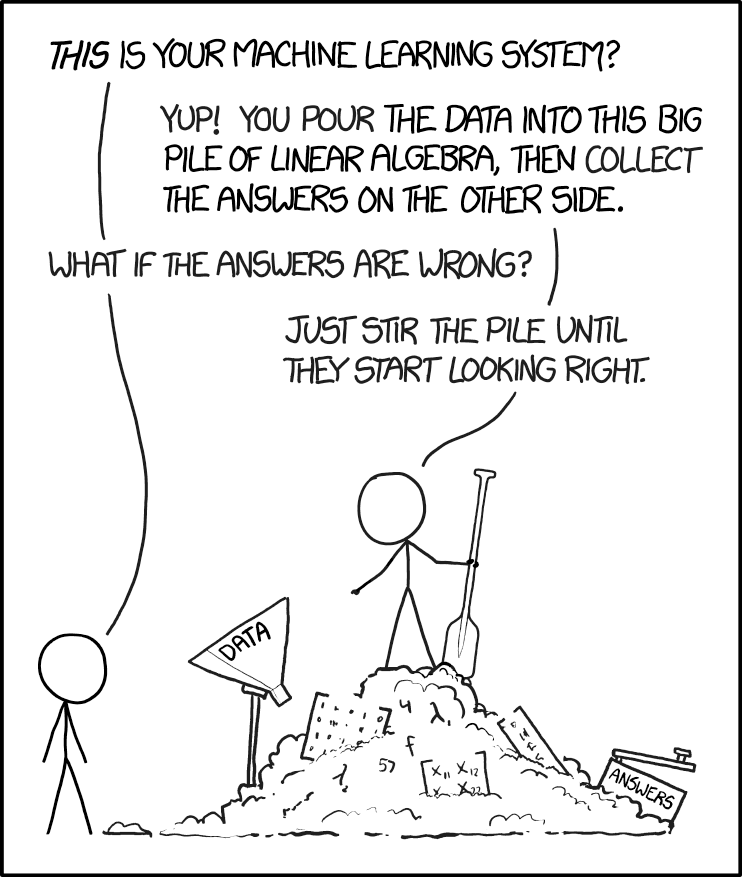
\includegraphics[height=.85\paperheight]{images/ml.png}
  \end{center}
\end{frame}

\begin{frame}
  \frametitle{Algebraic Reasoning}

\end{frame}

\begin{frame}
  \frametitle{Defining Data}

\end{frame}

\begin{frame}
  \frametitle{Dependent Types}

\end{frame}

\section{Conclusion}

\section{Questions?}
\end{document}
